%BEGIN TICKET 26
\begin{definition}
    $A \subset X$.  $A$ --- открытое множество, если  $\forall a \in A \exists B_r(a) \subset A$ ($r > 0$).
\end{definition}
\begin{theorem}[О свойствах открытых множеств]
    \begin{enumerate}
        \item $\emptyset, X$ --- открытые.
        \item Объединение любого числа открытых множеств --- открытое.
        \item Пересечение конечного числа открытых множеств --- открытое.
        \item $B_R(a)$ --- открытое.
    \end{enumerate}
\end{theorem}
\begin{proof}
    \begin{enumerate}
        \item[2.] $A_{\alpha}$ --- открытые,  $\alpha \in I$.  $B \eqqcolon \bigcup\limits_{\alpha \in I}A_{\alpha}$. Берем  $b \in B \implies b \in A_\beta$ для некоторого  $\beta$. Но  $A_\beta$ --- открытое  $\implies \exists r > 0\quad B_r(b) \subset A_\beta \subset B$.
        \item[3.] $A_1, A_2, \ldots, A_n$ --- открытые. $B \coloneqq \bigcap\limits_{k=1}^n A_k$. Берем  $b \in B \implies b \in A_k \forall k=1,2,\ldots,n$. Но $A_k$ --- открытое  $\implies \exists r_k > 0 B_{r_k} \subset A_k$. $\forall k\ B_{r_k}(b) \subset \bigcap\limits_{k=1}^n A_k = B \implies \exists r = \min\limits_{i = 1..k} r_k\!: B_r(b) \subset B\ \forall b \in B \implies B$ --- открытое.

         \item[4.] $\rho(a, x) < R$,  $r \coloneqq R - \rho(a, x) > 0$. Докажем, что  $B_r(x) \subset B_R(a)$. Возьмем  $y \in B_r(x)$, то есть  $\rho(x, y) < r \implies \rho(y, a) \le \rho(y, x) + \rho(x, a) < r + \rho(x, a) = R \implies y \in B_R(a)$.
    \end{enumerate}
             \begin{figure}[h!]
                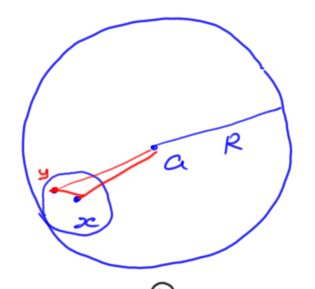
\includegraphics[width=0.25\textwidth]{open_set}
             \end{figure}
\end{proof}
\begin{remark}
    Существенна конечность. $\R$.  $\bigcap\limits_{n=1}^{\infty}(-\frac{1}{n}, 1) = [0, 1)$. А для нуля любой открытый шарик плохой.
\end{remark}
%END TICKET 26